\documentclass{article}
\usepackage{amsmath}
\usepackage{bm}
\usepackage{graphicx}
\usepackage[utf8]{inputenc}
\usepackage{caption}
\usepackage{subcaption}
\title{Planning. \\ Mathematical Modelling }
\author{Elisabeth Skaar Hasund}


\begin{document}
\maketitle

\section*{Synaptic cleft in 1D}

Diffusion equation in one dimension

\begin{equation}
u_t = \kappa u_{xx}.
\end{equation}

where $u$ is the concentration of neurotransmitters and $\kappa$ is the diffusion coefficient.

\subsection*{Scaling of variables}

\begin{align*}
\frac{\partial u^*}{\partial t^*} = \kappa \frac{\partial^2u^*}{\partial {x^*}^2}
\end{align*}

Use the scaling 

\begin{align*}
x^* &= L x \\
t^* &= T t \\
u^* &= N u 
\end{align*}

and replace in the diffusion equation s.t.

\begin{align*}
\frac{N}{T}\frac{\partial u}{\partial t} &= \kappa \frac{N^2}{L^2}\frac{\partial^2u}{\partial x^2} \\
\frac{\partial u}{\partial t} &= \eta \frac{\partial^2u}{\partial x^2}, & \eta = \kappa\frac{NT}{L^2}
\end{align*}

Using the values $L = 15 \cdot 10^{-9}$, $T = 10^{-4}$, $N = 5000$ and $\kappa = 0.3\cdot 10^{-12}$, we get the resulting value $\eta \approx 667$. 



\subsection*{Initial and boundary conditions}

The number of neurotransmitters released in one excitation is $N = 5000$. The number of receptor on one membrane is $R \approx \rho_R \cdot \pi r^2 \approx 152$ where $\rho_R$ is the density of receptors and $r$ is the radius of the synaptic cleft. Let $\Omega$ be the line between $0$ and $L$.

Initial values:

\[ u(x,0) = \left\{ 
  \begin{array}{l l}
    N & \text{if x = 0}\\
    0 & \text{elsewhere}
  \end{array} \right.\]

Neumann boundary conditions:

\begin{align*}
u_x(0,t) &= 0, \\
u_x(L,t) &= J(t)
\end{align*}

where $J(t)$ can be thought of as flux describing the rate of reaction in the chemical reaction
\begin{equation}
R + N \rightleftharpoons RN.
\end{equation}

The homogeneous Neumann boundary condition comes from the physical explanation that neurotransmitters cannot go back through the axon terminal.

\subsection*{Numerical scheme}

Using Crank-Nicholsons method, we obtain 

\begin{align*}
(1 - \frac{k}{2h^2} \delta^2_x)U^{n+1}_m = (1 + \frac{k}{2h^2} \delta^2_x) U_m^n
\end{align*}

where $k$ and $h$ are the time and space step, respectively. 

The resulting numerical scheme is

\begin{align*}
\left(I - \frac{r}{2} A\right) U^{n+1} = \left(I + \frac{r}{2} A\right) U^n
\end{align*}

where $r = \frac{k}{h^2}$,


\begin{align*}
A = 
\begin{pmatrix}
  -2 & 1 &  &  \\
  1 & \ddots & \ddots &  \\
    & \ddots  & \ddots & 1 \\
   &  & 1 & -2
\end{pmatrix} 
\textrm{ and }
U = \begin{pmatrix}
U_1 \\
U_2 \\
\vdots \\
U_{M} 
\end{pmatrix}
\end{align*}



Adding Neumann boundary conditions to the system, we expand the numerical scheme to involve boundary points, and an additional term

\begin{align*}
d^n = 
\begin{pmatrix}
0 \\
\vdots \\
0 \\
J^n
\end{pmatrix}
\end{align*}

such that the resulting scheme becomes

\begin{align*}
\left(I - \frac{r}{2} A\right)U^{n+1} = \left(I + \frac{r}{2} A\right) U^n + \frac{k}{2h}(d^n + d^{n+1}).
\end{align*}


\subsection*{Flux}

The rate of Neurotransmitters leaving the synaptic cleft can be described as a flux $J(t)$. Let $\Omega_{\epsilon}$ be a small area close to $L$ with width $\epsilon$, see Figure \ref{fig:model_1d}. Let $N_{\epsilon}(t)$ be the density of neurotransmitters in $\Omega_{\epsilon}$. These neurotransmitters are close enough to react with the receptors, and will affect the flux out of $\Omega$. Let $\rho_R$ be the density of receptors in the area $\epsilon$, and let $P^R(t)$ be the probability that one receptor is available. With reaction constants $k_1$ and $k_2$, the flux can be expressed as

\begin{align*}
J(t) = k_1 N_{\epsilon}(t) \rho_R P^R(t) - k_2 \rho_R (1-P^R(t)).
\end{align*}


\begin{figure}[ht]
        \centering
        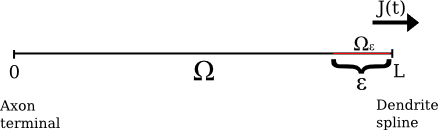
\includegraphics[clip=true,width=0.6\textwidth]{model_1d}
        \caption{Model of the synaptic cleft in one dimension}
        \label{fig:model_1d}
\end{figure}


\section*{Synaptic cleft in 2D}

A 2-dimensional model for the neurotransmitters diffusing from the axon terminal to the dendrite spine.

Let $L$ be the diameter and $b$ the height of the synaptic cleft. Assume that initially the neurotransmitters are uniformly distributed on the axon terminal, and the receptors are uniformly distributed on the dendritic spine. Assume that the surface of the dendritic spine is covered by an extracellular fluid 

CITATION

with thickness $\epsilon$. Like in the 1D-model, the neurotransmitters in this area can react with unoccupied receptors. 

Using the 5-point-formula, one can create a numerical scheme for the diffusion in 2 dimensions. This was attempted, but the system was numerically unstable, so it will not be included in this report. However, Matlab's ODE45 solver was applied to the same problem with success. 

\end{document}
